\section{Wavelets}
\subsection{Allgemein}
    Verbesserung der Short-Time-Fourier-Transformation: 
    \begin{liste}
        \item Die Breite des Fensters wird f�r jede Spektralkomponente separat
        berechnet (Skalierungsfunktion) 
        \item Die Fensterfunktion wird nicht transformiert
    \end{liste}

\subsection{Schnelle Wavelet-Transformation}
\begin{tabular}{ll}
\parbox{12.5cm}{
    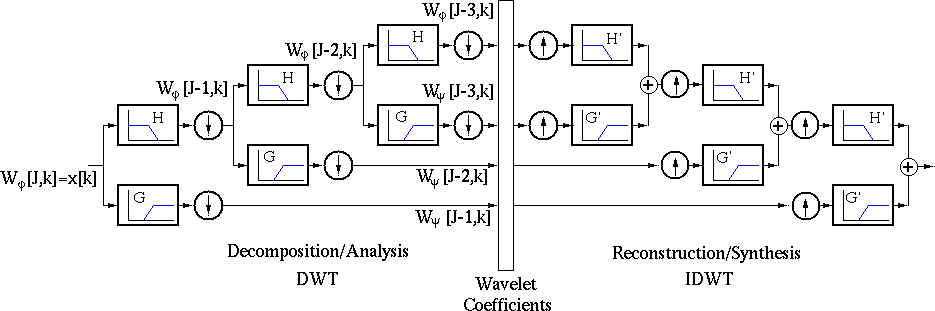
\includegraphics[width=12.5cm]{Content/Wavelet/wavelet-trafo.png}
	\begin{liste}
        \item Mit FFT vergleichbar (Bild oben)
        \item Auch ``Oktav-Zerlegung'' genannt
        \item Quadratur Mirror Filter: Tief- $H(z)$ \& Hochpass $G(z)$
        \item Up- \& Downsampling mit Faktor 2
    \end{liste}
    }
& \parbox{7cm}{
    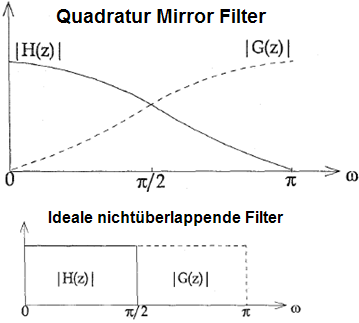
\includegraphics[width=6cm]{Content/Wavelet/wavelet-qmf.png}
    }
\end{tabular}

%\subsection{Vorgehen zur Bestimmung der Filterkoeffizienten}
%\begin{tabular}{ll}
%\parbox{14cm}{
	%\begin{aufzaehlung}
	 %\item Filterl�nge $L$ der FIR-Filter $H(z)$ bestimmen
	 %\item Grundgleichungen aufstellen:
	  %\begin{liste}
	    %\item $H(z) = \sum\limits_{n=0}^N h(n)z^{-n} = h(0) +
	    %h(1)z^{-1}+h(2)z^{-2}+\ldots$
	    %\item $G(z) = -z^{-N}H(-z^{-1})$
	    %\item $H'(z) = -z^{-N} H(z^{-1})$
	    %\item $G'(z) = z^{-N}G(z^{-1}) = -H(-z)$
	  %\end{liste}
	 %\item Gleichungssystem f�r Unbekannte $h(n)$ aufstellen. Bedingungen:
	  %\begin{liste}
	   %\item Perfekte Rekonstruktion (d.h. nur Verz�gerung): 
	     %$H(-z)H(-z^{-1}) + H(z)H(z^{-1}) = 2$
	   %\item $G(z)$ ist HP, darum: $G(e^{j0}) = G(1) = 0 = H(e^{j\pi}) = H(-1)$
	   %\item Wenn noch Freiheitsgrade vorhanden: Methode \textit{Daubechies}:
	   %``Smoothe Wavelets'' durch $\dfrac{\delta^p G'(1)}{\delta \omega^p} = 0$,
	   %wobei $p = 1..$(Anzahl restlichen Freiheitsgrade)
	  %\end{liste}
	%\end{aufzaehlung}
	%}
%& \parbox{4cm}{
    %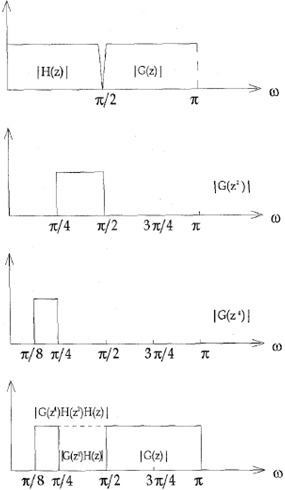
\includegraphics[width=3.7cm]{Content/Wavelet/wavelet-spektrum.png}}
%\end{tabular}